% Document class
\documentclass{beamer}
\usecolortheme{default}
\usetheme{Madrid}
\usepackage{graphicx}
\usepackage{subfigure}
\usepackage{comment}
\usepackage{enumitem}

% Preamble
\title{Multivariate Time Series Modelling Of Ex-Pump Prices Of Petroleum Products In Ghana}
\subtitle{Chapter 4: Results and Discussions}
\author{Group 41}
\institute{Kwame Nkrumah University of Science and Technology}
\subject{Final Year Project}
\logo{
\includegraphics[width=20pt, height=20pt]{images/logo/logoKnust.png}}
\date{\today}

% Customizing table of contents
\setbeamertemplate{section in toc}[sections numbered]
\setbeamertemplate{subsection in toc}[subsections numbered]
\setbeamercolor{section in toc}{fg=blue}
\setbeamercolor{subsection in toc}{fg=blue!70}

% Define variables
\newcommand{\startDate}{January, 2007 }
\newcommand{\finishDate}{June, 2015 }
\newcommand{\numOfObservations}{204 }

\newcommand{\vspaceFive}{\vspace{5pt}}
\newcommand{\vspaceTen}{\vspace{10pt}}
\newcommand{\hspaceFive}{\hspace{5pt}}
\newcommand{\colorHighlight}{blue}
\newcommand{\warning}{red}
\newcommand{\textHighlight}[1]{\textcolor{blue}{#1}}

\newcommand{\VAR}{Vector Autocorelation }
\newcommand{\VARHighlight}{\textHighlight{Vector Autocorelation }}
\newcommand{\VEC}{Vector Error Correlation }
\newcommand{\VECHighlight}{\textHighlight{Vector Error Correlation }}





% Body
\begin{document}
	
	% Insert title here
	\begin{frame}
		\titlepage
	\end{frame}

	% Insert table of content
	\begin{frame}{Table of Contents}
		\tableofcontents
		
	\end{frame}
	
	% --------------------------------------------------------------------
	% Introduction
	% --------------------------------------------------------------------
	\section{Introduction}
	\begin{frame}{Introduction}
		
		\begin{block}{Objective}
			The purpose of the study is to obtain a suitable model for the ex-pump prices of petroleum products in Ghana. 
		\end{block} \vspace{5pt}
		
		 To examines how changes in the prices of one product cause changes in the price of others in both the short and long terms. \par \vspace{5pt}
		
		Data spanning \startDate to \finishDate are obtained from the National Petroleum Authority of Ghana, covering four petroleum products; \textHighlight{Gasoline, Gasoil, Kerosene, and Liquefied Petroleum Gas (LPG) }. 
	\end{frame}
	
	% --------------------------------------------------------------------
	\begin{frame}{Chapter 4: Result And Discussion}
		This chapter analyses and discusses the results. It presents results of the association between the prices of the products considered, namely; \vspace{5pt}
		
		\begin{itemize}
			\item Gasoil
			\item Gasolin
			\item Kerosene 
			\item Liquefied Petroleum Gas (LPG)
		\end{itemize} \vspace{5pt}
		
		All associated tests and models are generated with R 
	\end{frame}
	
	% --------------------------------------------------------------------
	% Descriptive Statistics
	% --------------------------------------------------------------------
	\section{Descriptive Statistics}
	\begin{frame}{Descriptive Statistics}
		\begin{block}{}
			\vspace{4pt}
			In all, \numOfObservations observations are used (\startDate to \finishDate). \vspace{4pt}
		\end{block} \vspace{5pt}
		
		\begin{block}{}
		Training data of 144 observations (January 2007 to December 2012) for modelling \\ \vspace{5pt}
		
		Testing data of 60 data points (January 2013 to June 2015) for model validations.
		\end{block} \vspace{5pt}
	
		\begin{block}{}
			The descriptive statistics of the products are shown in Table \ref{table:description} on page \pageref{table:description}
		\end{block}
	\end{frame}
	
	% --------------------------------------------------------------------
	\begin{frame}{Summary Statistics}
		\begin{table}[]
			\caption{ \ref{table:description} Summary Statistics}
			\begin{tabular}{lllll}
\hline
Statistics             & GASOIL  & GASOLINE & KEROSENE & LPG     \\ \hline
Mean                   & 122.445 & 123.570  & 82.989   & 94.766  \\
Maximum                & 175.480 & 177.090  & 120.420  & 136.190 \\
Minimum                & 11.600  & 49.170   & 6.470    & 58.500  \\
Standard Deviation     & 32.306  & 31.817   & 27.186   & 20.609  \\ 
Skewness               & -0.201  & 0.1307   & -1.988   & 0.413   \\
Kurtosis               & 3.374   & 2.123    & 6.293    & 2.292   \\
Number of Observations & 144     & 144      & 144      & 144     \\ \hline
			\end{tabular}
			\label{table:description}
		\end{table}
	\end{frame}

	% -------------------------------------------------------------------
	\begin{frame}{Plot of Original Series}
		\begin{figure}
			\subfigure{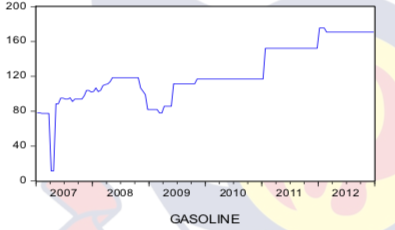
\includegraphics[height=0.3\textheight, width=0.4\textwidth]{images/plots/plot_original/plot_original_gasoline}}
			\subfigure{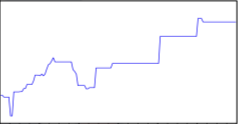
\includegraphics[height=0.3\textheight, width=0.4\textwidth]{images/plots/plot_original/plot_original_gasoil}}
			\subfigure{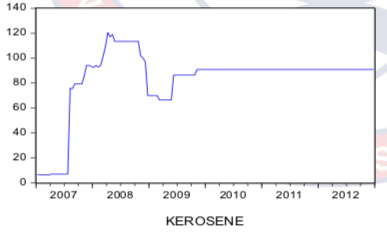
\includegraphics[height=0.3\textheight, width=0.4\textwidth]{images/plots/plot_original/plot_original_kerosene}}
			\subfigure{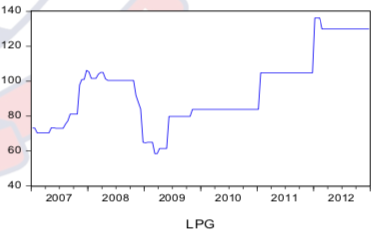
\includegraphics[height=0.3\textheight, width=0.4\textwidth]{images/plots/plot_original/plot_original_lpg}}
			
			
			\caption{ \ref{plot:original_series} Time Series Plot of the Original Series}
			\label{plot:original_series}
		\end{figure}
		
	\end{frame}
	
	% --------------------------------------------------------------------
	% Trend and Stationarity Test
	% --------------------------------------------------------------------
	\section{Stationarity Test}
	
	\begin{comment}
	\begin{frame}{Trend Test}
		For trend test, We have chosen to apply
		
		\begin{block}{ Mann-Kendall Test}
			H0 : There is no monotonic trend in the dataset over time. \\
			H1 : There is a monotonic trend in the dataset over time. \vspace{5pt}
		\end{block}
		
		\begin{exampleblock}{Sen's Slope Test}
			H0 : There is no tonic trend in the dataset over time. \\
			H1 : There is a tonic trend in the dataset over time. \vspace{5pt}
		\end{exampleblock}
	\end{frame}
	\end{comment}

	\begin{frame}{Staionarity Test}
		We have numerous ways of testing for the presence of a unit root. 
		We have chosen to apply
		
		\begin{block}{Augmented Dickey-Fuller Test}
			H0 : The series is not stationary \\
			H1 : The series is stationary. \vspace{5pt}
		\end{block}
	
		\begin{exampleblock}{Phillips-Perron Unit Root Test}
			H0 : The series is not stationary \\
			H1 : The series is statrionary. \vspace{5pt}
		\end{exampleblock}
		
		\begin{alertblock}{KPSS Test for Level Stationarity}
			H0 : The series is stationary \\
			H1 : The series is not statrionary. \vspace{5pt}
		\end{alertblock}
	\end{frame}
	
	% --------------------------------------------------------------------
	\begin{frame}{Stationarity of Original Series}
		\begin{table}[]
			\caption{ \ref{table:stationarity_original} Univariate URTs of the Original Series}
			\label{table:stationarity_original}
			\begin{tabular}{llllll}
\hline
&  & \multicolumn{2}{l}{(Test Statistics)} & \multicolumn{2}{l}{(P-Values)} \\ \hline

SERIES   & LAG ORDER & ADF    & KPSS      & ADF    & KPSS           \\

GASOLINE & 5         & -2.738 & 2.370     & 0.269  & 0.010          \\

GASOIL   & 5         & -2.450 & 2.437     & 0.389  & 0.010          \\

KEROSENE & 5         & -3.106 & 0.709     & 0.166  & 0.010          \\

LPG      & 5         & -1.975 & 1.497     & 0.587  & 0.010          \\ \hline
			\end{tabular}
		\end{table}
	
	\begin{alertblock}{Is Stationary ?}
		\vspace{5pt}
		It is observed that for ADF, all the p-values of the series are greater than 0.05 and this indicates non stationarity. The KPSS test also showed the same results. We now  difference the series since the series are not stationary.
	\end{alertblock}
	\end{frame}
	
	% --------------------------------------------------------------------
	% Differencing
	% --------------------------------------------------------------------
	\section{Differencing}
	\begin{frame}{Differencing}

			\begin{alertblock}{First Difference}
				\vspace{5pt}
				Since all the series (Gasoline, Gasoil, Kerosene, LPG) are not stationary we perform 1st differencing in order to achieve stationarity;
				The figure \ref{plot:difference_series} below is a plot after the first differencing .
				\vspace{5pt}
			\end{alertblock}
		
	\end{frame}
	
	% --------------------------------------------------------------------
	\begin{frame}{Plot of First Differenced Series}
		\begin{figure}
			\subfigure{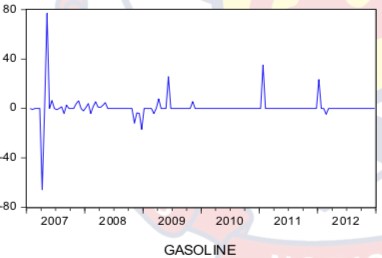
\includegraphics[height=0.3\textheight, width=0.4\textwidth]{images/plots/plot_diff/plot_diff_gasoline}}
			\subfigure{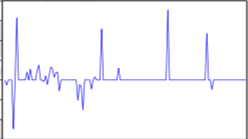
\includegraphics[height=0.3\textheight, width=0.4\textwidth]{images/plots/plot_diff/plot_diff_gasoil}}
			\subfigure{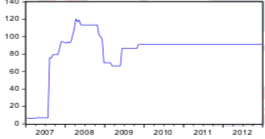
\includegraphics[height=0.3\textheight, width=0.4\textwidth]{images/plots/plot_diff/plot_diff_kerosene}}
			\subfigure{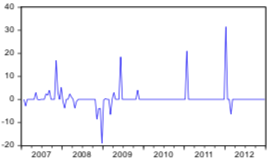
\includegraphics[height=0.3\textheight, width=0.4\textwidth]{images/plots/plot_diff/plot_diff_lpg}}
			
			
			\caption{ \ref{plot:difference_series} Time Series Plot of the Original Series}
			\label{plot:difference_series}
		\end{figure}
		
	\end{frame}

	% --------------------------------------------------------------------
	\begin{frame}{Stationarity of First Differenced Series}
		\begin{table}[]
			\caption{ \ref{table:stationarity_first_diff} Univariate URTs of the Differenced Series}
			\label{table:stationarity_first_diff}
			\begin{tabular}{llllll}
	\hline
	&  & \multicolumn{2}{l}{(Test Statistics)} & \multicolumn{2}{l}{(P-Values)} \\ \hline
	SERIES   &LAG ORDER & ADF    & KPSS      & ADF    & KPSS           \\
	
	GASOLINE &5         & -7.781 & 0.031     & 0.010  & 0.10          \\
	
	GASOIL   &5         & -5.537 & 0.045     & 0.010  & 0.10          \\
	
	KEROSENE &5         & -4.493 & 0.263     & 0.010  & 0.10          \\
	
	LPG      &5         & -4.473 & 0.063     & 0.010  & 0.10          \\ \hline
			\end{tabular}
		\end{table}
	
		\begin{exampleblock}{Is Stationary ?}
			\vspace{5pt}
			It is observed that for ADF, all the p-values of the series are less than 0.05 and this
			indicates the stationarity. The KPSS test also showed the same results. We now estimate the models since the series have attained stationarity.
		\end{exampleblock}
	\end{frame}

	% --------------------------------------------------------------------
	\begin{frame}{ACF Plot of First Differenced Series}
		\begin{figure}
			\subfigure{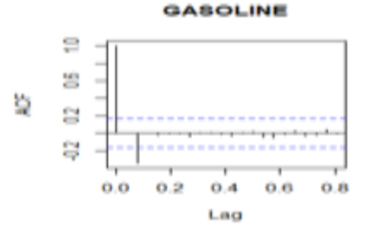
\includegraphics[height=0.3\textheight, width=0.4\textwidth]{images/acf_pacf/acf_pacf_diff/acf_diff_gasoline}}
			\subfigure{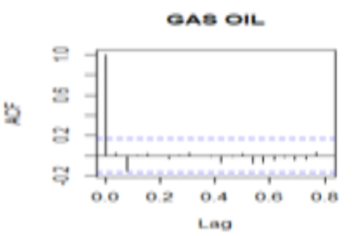
\includegraphics[height=0.3\textheight, width=0.4\textwidth]{images/acf_pacf/acf_pacf_diff/acf_diff_gasoil}}
			\subfigure{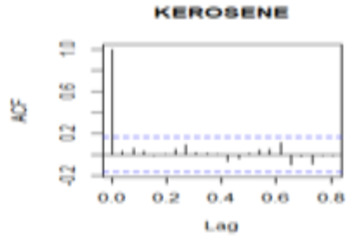
\includegraphics[height=0.3\textheight, width=0.4\textwidth]{images/acf_pacf/acf_pacf_diff/acf_diff_kerosene}}
			\subfigure{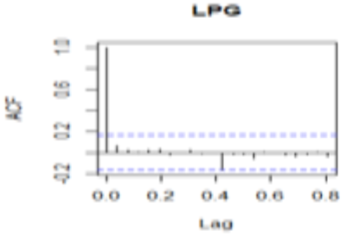
\includegraphics[height=0.3\textheight, width=0.4\textwidth]{images/acf_pacf/acf_pacf_diff/acf_diff_lpg}}
			
			
			\caption{ \ref{plot:acf__diff_series} ACF of the Differenced Series}
			\label{plot:acf__diff_series}
		\end{figure}
		
	\end{frame}
	
	% --------------------------------------------------------------------
	\begin{frame}{PACF Plot of First Differenced Series}
		\begin{figure}
			\subfigure{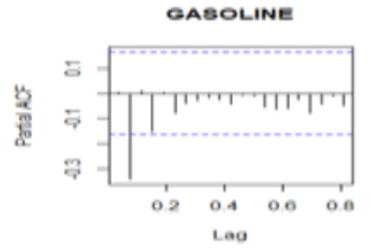
\includegraphics[height=0.3\textheight, width=0.4\textwidth]{images/acf_pacf/acf_pacf_diff/pacf_diff_gasoline}}
			\subfigure{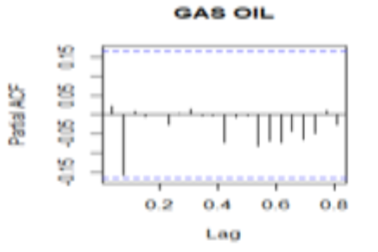
\includegraphics[height=0.3\textheight, width=0.4\textwidth]{images/acf_pacf/acf_pacf_diff/pacf_diff_gasoil}}
			\subfigure{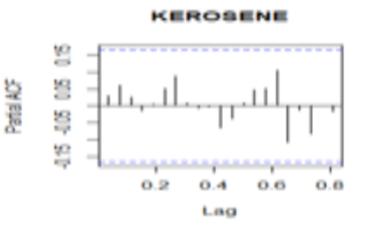
\includegraphics[height=0.3\textheight, width=0.4\textwidth]{images/acf_pacf/acf_pacf_diff/pacf_diff_kerosene}}
			\subfigure{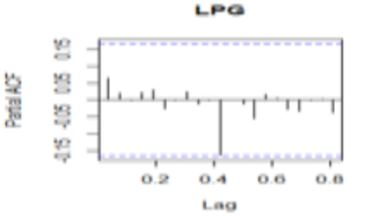
\includegraphics[height=0.3\textheight, width=0.4\textwidth]{images/acf_pacf/acf_pacf_diff/pacf_diff_lpg}}
			
			
			\caption{ \ref{plot:pacf__diff_series} PACF of the Differenced Series}
			\label{plot:pacf__diff_series}
		\end{figure}
		
	\end{frame}	
	
	
	% --------------------------------------------------------------------
	% Estimation of VAR or VEC Models
	% --------------------------------------------------------------------
	\section{Estimation of VAR/ VEC Models}
	\begin{frame}{Estimation of VAR/ VEC Models}
		\begin{block}{}
			Estimating parameters of \VARHighlight (VAR) or \VECHighlight (VEC) models require that variables are 
			covariance stationary \vspaceFive
		\end{block} \vspaceFive
		
		\begin{block}{}
			VAR for instance cannot be used if the variables are not stationary. \\
			Also, if the data is non-stationary, the forecast cannot be done because \textHighlight{VAR assumes stationarity}
		\end{block}
	
		\begin{block}{}
			We then test for the long run relationship using \textHighlight{Johansen’s cointegration test}.  \\
			That is if the result confirms that there is a long-run relationship among the variables, 
			we can proceed to the VEC model. 
		\end{block}
	
		\begin{exampleblock}{}
			The first step involved in estimating is to first determine the lag Length or order. 
		\end{exampleblock}
	\end{frame}

	% --------------------------------------------------------------------
	\begin{frame}{Estimation of VAR/ VEC Models }
		
		\begin{block}{What Next After Series is Stationary ?}
			\vspaceFive
			\begin{itemize}[label=$\diamond$, leftmargin=2em, itemsep=1em]
				\item Lag Length Selection (LLS)
				\item Cointegration Test
				\item Long Term Equilibrium
				\item Short Term Equilibrium
				\item Estimation of VEC Model (If There is cointegration)
				\item Model Validation
				\item Forecast of Ex-Pump prices of Products
			\end{itemize}
			\vspaceFive
		\end{block}
		
	\end{frame}

	
	% --------------------------------------------------------------------
	% LLS Criteria and Cointergration
	% --------------------------------------------------------------------
	
	% --------------------------------------------------------------------
	% Long and Short Term Equilibrium
	% --------------------------------------------------------------------
	
	% --------------------------------------------------------------------
	% Estimation of VEC Model
	% --------------------------------------------------------------------
	
	% --------------------------------------------------------------------
	% Model Validation
	% --------------------------------------------------------------------
	
	% --------------------------------------------------------------------
	% Forecast of Ex-Pump Prices of Products
	% --------------------------------------------------------------------
	
	% --------------------------------------------------------------------
	% Granger Gausality Test
	% --------------------------------------------------------------------
	
	% --------------------------------------------------------------------
	% Impurse Response Functions ( IRFs )
	% --------------------------------------------------------------------
	
	% --------------------------------------------------------------------
	% Summary of Results
	% --------------------------------------------------------------------
	
	% --------------------------------------------------------------------
	% Summary of Chapter
	% --------------------------------------------------------------------
	
	
	
\end{document}